\documentclass{article}
\usepackage{spconf,amsmath,graphicx}

\usepackage{color}
\usepackage{balance}
\linespread{1}
% dblfloatfix

\def\x{{\mathbf x}}
\def\L{{\cal L}}

% Title.
% ------
\title{Thickness profile measurement between closed curves}
\name{Mat\'ias Tailani\'an, Federico Lecumberry}
\address{Facultad de Ingenier\'ia, Universidad de la Rep\'ublica\\
	 Julio Herrera y Reissig 565, Montevideo, Uruguay
}

\begin{document}
\maketitle

\begin{abstract}
In this paper the problem of defining and measuring a thickness profile between closed curves is presented. Based on the normal evolution of curves, we developed an algorithm that defines the correspondence between points of different curves and measures the thickness profile. Ensuring in each step a good sampling of all curves by mechanisms of creating and deleting points, the algorithm splits the evolution in two parts, evolving from the convex hull of the interior curve to each one of the others. Synthetic and real results are shown and a particular application of classification using descriptors extracted from the thickness profile is presented.
\end{abstract}

\begin{keywords}
Curves evolution, thickness, distance, endometritis
\end{keywords}

\section{Introduction}
\label{sec:intro}
This work addresses the problem of finding an entire thickness profile between two closed curves. The particular application considered is to detect a common uterine disease in dairy cattle using ultrasonographic images. An expert in ultrasonographic diagnosis affirms (Giovanni Gnemmi, personal communication, May 18th, 2013) that the relation between some muscles thickness can be a relevant characteristic to diagnostic this disease. In this work we explore this possibility developing a system to measure this feature. Figure \ref{fig:defs}a shows a typical setting of the closed curves involved in the problem: $\Gamma_1$, $\Gamma_2$, $\Gamma_3$. Curves are always in this order and there is no intersection between them, since they are the limits of muscles and tissues in cattle uterus. $\Gamma_1$ and $\Gamma_2$ are not assumed to be convex but presents a smooth curvature variation, while $\Gamma_3$ is non convex, with high curvature variation and even not differentiable in some points. The main goal is to define and measure the thickness profile of the muscles, which means to find the thickness of the region between $\Gamma_1$ and $\Gamma_2$, and between $\Gamma_2$ and $\Gamma_3$. In the literature there are some measures of distance between two curves, such as Housedorff \cite{libroMorel}, or Sobolev \cite{statistics}, providing a numeric value for the distance or dissimilarity between curves, but we are interested, as said, in the entire thickness profile. Several methods, like the one presented in \cite{paperWarping}, finds the correspondence between two morphologically different objects by the minimization of a similarity criterion function. Other methods resolve the correspondence by circle mapping \cite{libro}: the vertices of the source and target curves are projected on circles of the same radius, and then merged. The merged set of vertices are projected back onto each curve, obtaining curves with the same number of vertices, and in a pairwise correspondence.

To compute the thickness of a region, the first question to ask is how to conceptually define the width between two curves. It is clear that is a local characteristic that depends of at least two points in different curves. The distance function for each point of a curve to the other curve leads to a non-intuitive definition of width, see Figure \ref{fig:comp}. In this work we propose an algorithm based on the normal evolution of one curve and considering the other curve as target. In the evolution are included some mechanisms of creating and deleting points to ensure a correct sampling of the curves at all steps. The width is measured as the length of the path in the evolution from one curve to the other. This algorithm finds an intuitive correspondence between points of the different curves and leads to an appropriate width definition.

The description of the particular problem considered and the proposal is presented in Section \ref{sec:proposal}. In Section \ref{sec:results} are presented synthetic and real results and a final application to diagnostic an uterine disease using descriptors extracted from the thickness profile. Finally, in Section \ref{sec:conc} we present some conclusions and future work.

\begin{figure}[t]
\begin{minipage}[b]{.45\linewidth}
  \centering
  \centerline{
\includegraphics[width=3.8cm]{pics/defs2}}
  \centerline{(a)}\medskip
\end{minipage}\hfill
\begin{minipage}[b]{.52\linewidth}
  \centering
  \centerline{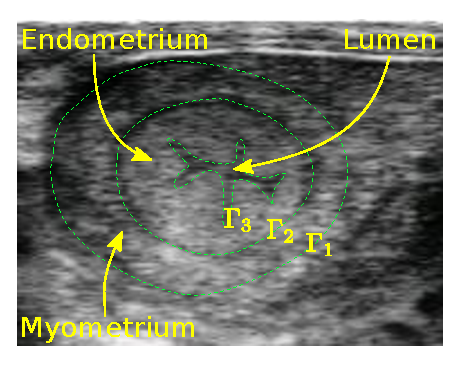
\includegraphics[width=4.2cm]{pics/defsEndo}}
  \centerline{(b)}\medskip
\end{minipage}
\caption{Definitions. A schematic representation of the problem is shown in (a), while in (b) is presented a real example of the application. The region between $\Gamma_1$ and $\Gamma_2$ is called \emph{Myometrium}, the region between $\Gamma_2$ and $\Gamma_3$ \emph{Endometrium} and the region inside $\Gamma_3$ \emph{Lumen}.}
\label{fig:defs}
\end{figure}

\section{Problem description and proposal}
\label{sec:proposal}

\subsection{Problem description}
\label{ssec:description}
In order to understand the particular application considered it is important to define some concepts. In Figure \ref{fig:defs}b a transverse cut of cattle uterine horn is shown. We can imagine the uterine horn as a tube with two coatings: Endometrium and Myometrium. The Myometrium is the region delimited by $\Gamma_1$ and $\Gamma_2$ and the Endometrium is the region delimited by $\Gamma_2$ and $\Gamma_3$. The problem is to measure the thickness of those two regions, using a manual segmentation of the regions.
\begin{figure*}[t]
\begin{minipage}[b]{.32\linewidth}
  \centering
  \centerline{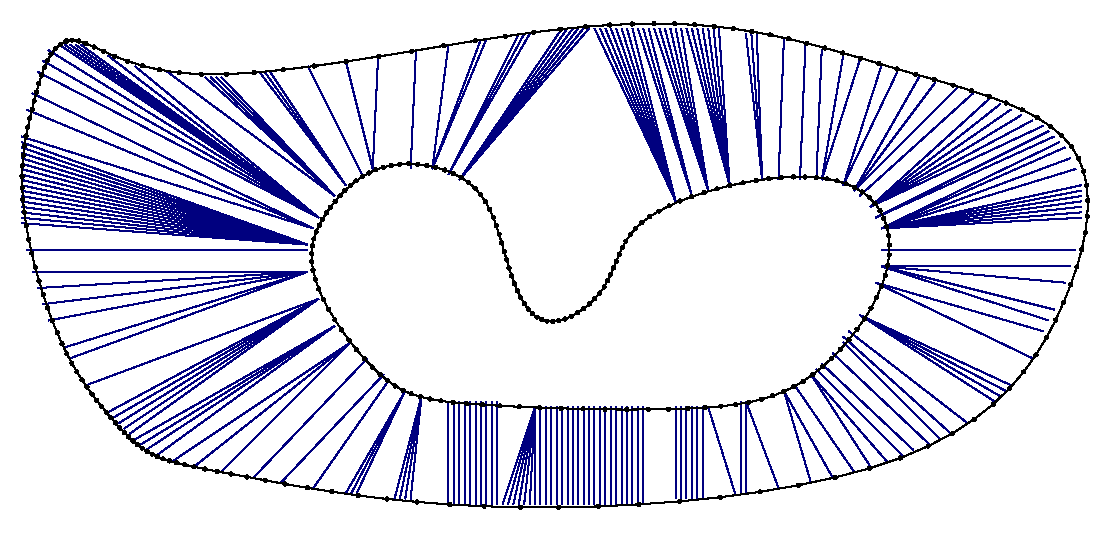
\includegraphics[width=5.8cm]{pics/cmp_dist}}
  \centerline{(a)}\medskip
\end{minipage}
\hfill
\begin{minipage}[b]{.32\linewidth}
  \centering
  \centerline{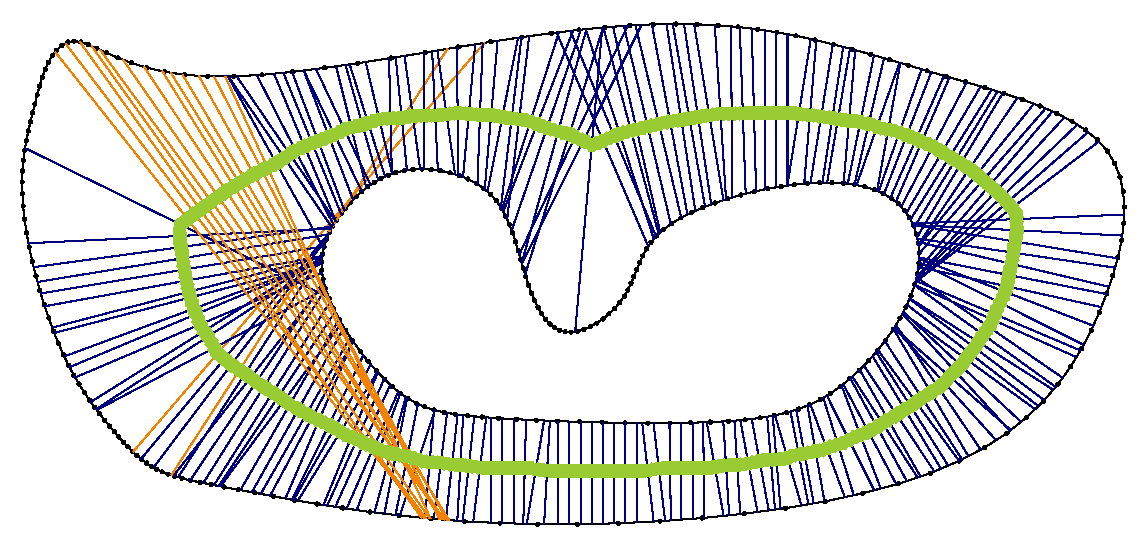
\includegraphics[width=5.8cm]{pics/cmp_norm2}}
  \centerline{(b)}\medskip
\end{minipage}
\hfill
\begin{minipage}[b]{.32\linewidth}
  \centering
  \centerline{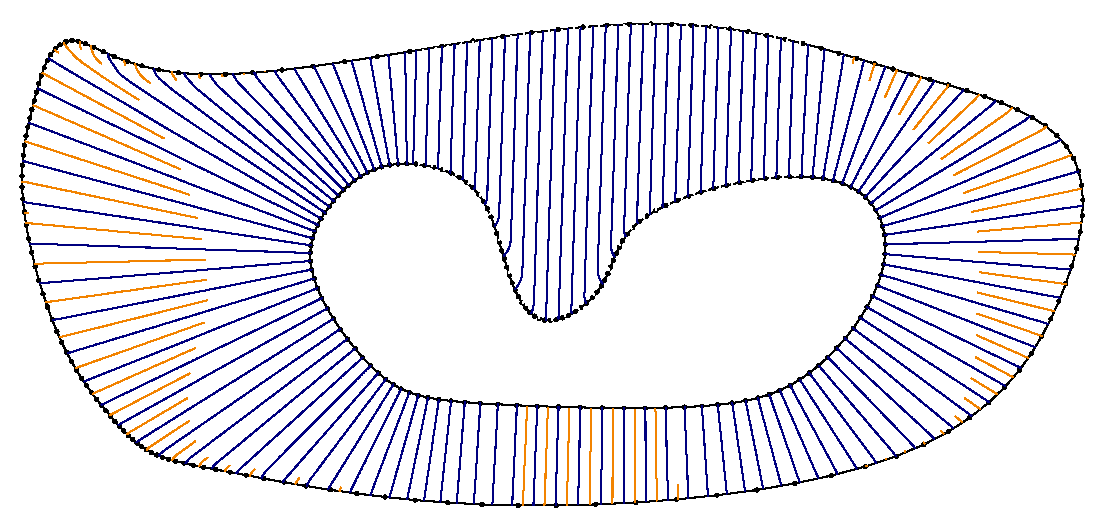
\includegraphics[width=5.8cm]{pics/cmp_evol}}
  \centerline{(c)}\medskip
\end{minipage}
\caption{Comparison between different proposals. (a) Distance function from the points in the outer curve to the inner curve. (b) Defining the middle curve as the curve equidistant to both curves, the thickness is measured as the length of the normal to the middle curve. (c) Proposal: the blue lines represent the path traveled by the original points during evolution, and the orange lines corresponds to points created during evolution, see Section \ref{sec:proposal}.}
\label{fig:comp}
\end{figure*}
While searching for a definition of the distance between two curves, euclidean distance comes to head. In this case, for each point of curve $\Gamma_i$ the nearest point of $\Gamma_j$ is found and the euclidean distance between this two points is used as thickness. As can be seen in Figure \ref{fig:comp}a, this thickness definition cannot capture the curves ``structure'', deriving in a wrong profile. Another idea is to measure width in the normal direction of each point of the curve. Considering the normal to curve $\Gamma_2$, we cannot ensure that this direction will intersect $\Gamma_3$. With the purpose of obtaining a more regular curve and define the thickness in the normal direction of this new curve, we consider the skeleton of the region defined by $\Gamma_2$ and $\Gamma_3$, defined as the curve $\Gamma_{23}$ equidistant to both curves. The results of measuring the thickness in the normal direction of each point of $\Gamma_{23}$ are not as expected and in some directions the normals do not intersect curve $\Gamma_3$ (See Figure \ref{fig:comp}b). Finally, in Figure \ref{fig:comp}c is presented our proposed algorithm. In this case, the ``structure'' of the curves are effectively captured, obtaining a distance between curves that can be interpreted as thickness.

Another possibility is to create synthetic images from the given curves in order to use other methods like GAC \cite{gac} o Chan-Vese \cite{chan-vese}, that uses image data to perform the evolution. However, this methods introduce other terms representing for example the curve regularity or area measures that are not linked to the original problem and may hinder the real problem of measuring a region thickness. 

\subsection{Proposal}
\label{ssec:proposal}
Our proposal is based on the simplest curves evolution: the normal evolution. Letting $\eta$ be the evolution step and $\vec{n}_{p_i}^t$ the normal to the curve at the point $p_i$ at time $t$, the evolution is governed by the equation:
\begin{equation}
  p_i^{t+1}=p_i^t+\eta \; \vec{n}_{p_i}^t.
  \label{ec:normal}
\end{equation}

Due to the nature of the curves described in Section \ref{sec:intro}, considering the non convexity of the curves, we propose to perform a two step evolution, which in the final step are joined to obtain a single result. Assuming that $\Gamma_3$ is non convex, an auxiliary curve is considered: the convex hull of curve $\Gamma_3$ ($\Gamma_3^{CH}$), \cite{libro}. The two steps of the evolution are:
\begin{enumerate}
  \item Evolution from $\Gamma_3^{CH}$ to $\Gamma_3$
  \item Evolution from $\Gamma_3^{CH}$ to $\Gamma_2$
\end{enumerate}
The final width, or distance between curves, is calculated as the distance of the path traveled by each point of the curve. The original curves are created with a cubic interpolation of a few points indicated by the expert and then re-sampled according to curvature, using more points in regions with higher curvature. The sampling of $\Gamma_3^{CH}$ is done by two different ways according to each point nature: points $p_i\in\Gamma_{3}$ that also belongs to $\Gamma_3^{CH}$ are directly used, and in regions where $\Gamma_3$ do not match $\Gamma_3^{CH}$, an uniform sampling is performed such that both curves have the same number of points.

Sampling conditions are considered at each step to ensure a correct representation of the curve. For that purpose we developed a simple mechanism of creating and deleting points while evolving the curve. At the beginning of the evolution, the mean distance, $\delta$, between adjacent points is computed. The procedure of creating new points consists on evaluating at each evolution step $t$ if the distance between two adjacent points $p_i^t$ and $p_{i+1}^t$ is greater than $2\delta$. In this case, a new point, $p_k^t$, is created between $p_i^t$ and $p_{i+1}^t$ as the middle point. $p_k^t$ is initialized with the mean of the distance traveled by points $p_i^t$ and $p_{i+1}^t$, see Figure \ref{fig:nacimiento_y_muerte}a. The procedure to combine points is based on the evaluation of a proximity condition. If $\eta\frac{\vec{n}_{p_i}}{||\vec{n}_{p_i}||}$ and $\eta\frac{\vec{n}_{p_i+1}}{||\vec{n}_{p_i+1}||}$ are intersected, points $p_i$ and $p_{i+1}$ will be joined into a new one, placed in that intersection, see Figure \ref{fig:nacimiento_y_muerte}b.
\begin{figure}[t]
\begin{minipage}[b]{.5\linewidth}
  \centering
  \centerline{
\includegraphics[width=4.3cm]{pics/nacimiento}}
  \centerline{(a)}\medskip
\end{minipage}
\hfill
\begin{minipage}[b]{.48\linewidth}
  \centering
  \centerline{
\includegraphics[width=3.7cm]{pics/muerte}}
  \centerline{(b)}\medskip
\end{minipage}
\caption{Mechanisms of creating and combining points during evolution. (a) A new point is created (red point) if the distance between adjacent points exceeds a predefined threshold. (b) Two points are combined if their normals normalized and multiplied by the step length intersect each other.}
\label{fig:nacimiento_y_muerte}
\end{figure}
%If the curvature of curve $\Gamma_2$ is very high, the procedure should change a little, considering the convex hull of $\Gamma_2$ and perfoming the same procedure as the described for $\Gamma_3$.
% tengo que decir como se mide la normal: con un vecino de cada lado.

\section{Results}
\label{sec:results}

\subsection{Synthetic}
\label{ssec:syn}
In order to show the algorithm performance, a synthetic example is presented. This example was designed considering $\Gamma_i$, $i=1\dots3$ as three concentric circles and adding a perturbation in $\Gamma_2$. This perturbation is introduced by adding in the normal direction of each point of the curve a Gaussian distribution $X \sim \mathcal{N}(0,1)$ centered in points with null phase. In the point where $X$ is maximal (null phase), the width of the region delimited by $\Gamma_1$ and $\Gamma_2$ is equal to the width of the region delimited by $\Gamma_2$ and $\Gamma_3$. The results are shown in Figure \ref{fig:synth}. Figure \ref{fig:synth}a shows the trajectory of the points while evolving. The trajectory of the original points is represented in blue color, while the trajectory of points created during evolution is represented in orange color. Figure \ref{fig:synth}b shows the thickness profile obtained relative to the angle measured from the center of the circles. As can be seen, the results are as expected. Region between $\Gamma_1$ and $\Gamma_2$ presents a decay in width while the region between $\Gamma_2$ and $\Gamma_3$ shows an increase. For the points with null phase the widths are equal.
\begin{figure}[t]
\begin{minipage}[b]{1\linewidth}
  \centering
  \centerline{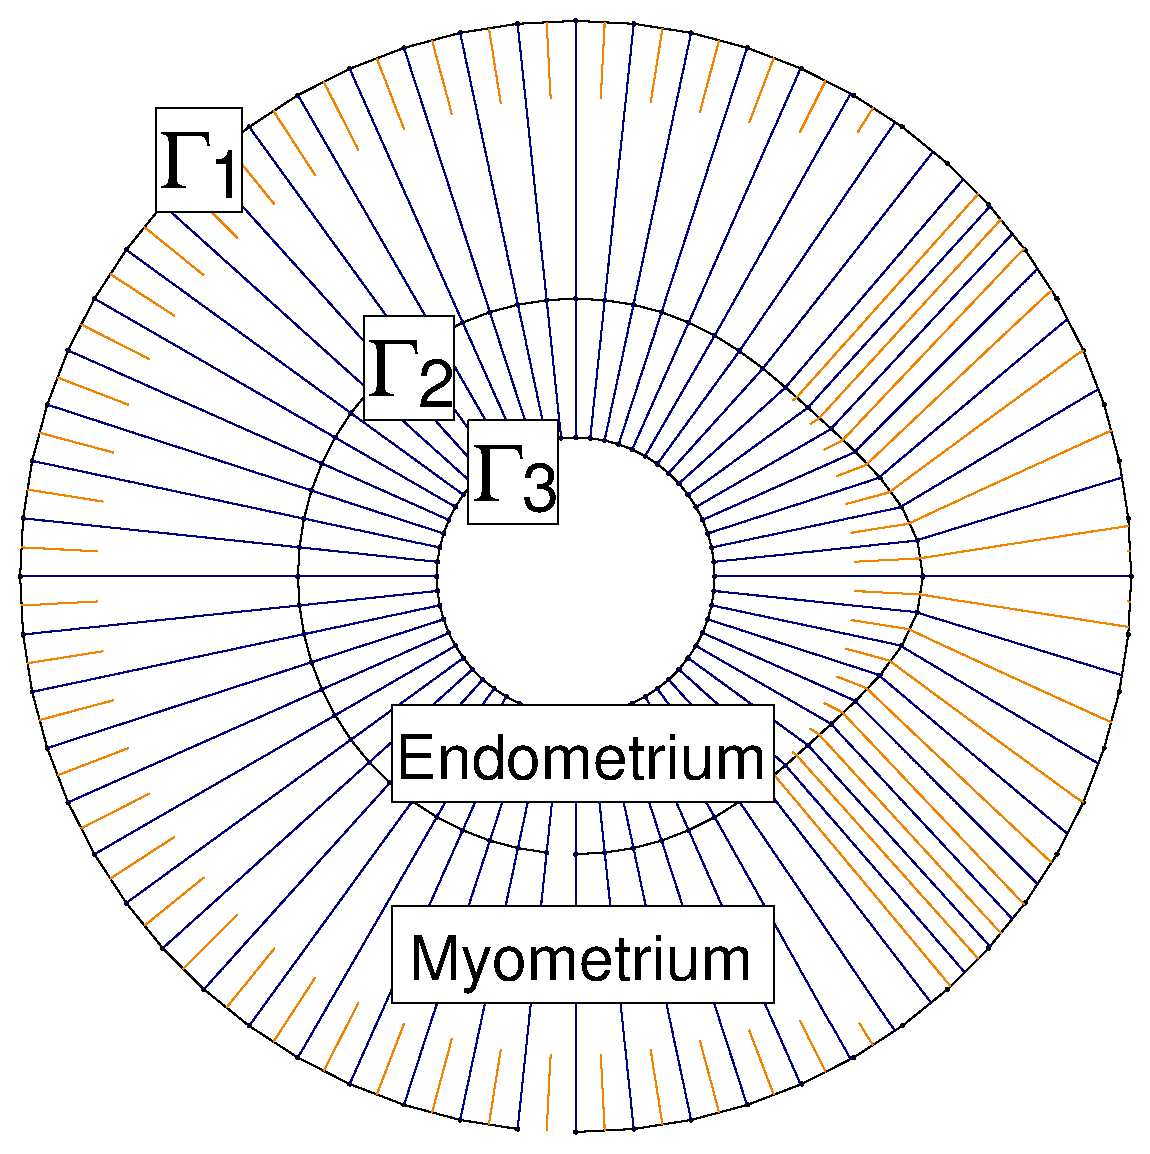
\includegraphics[width=5cm]{pics/synth}}
  \centerline{(a)}\medskip
\end{minipage}
\begin{minipage}[b]{1\linewidth}
  \centering
  \centerline{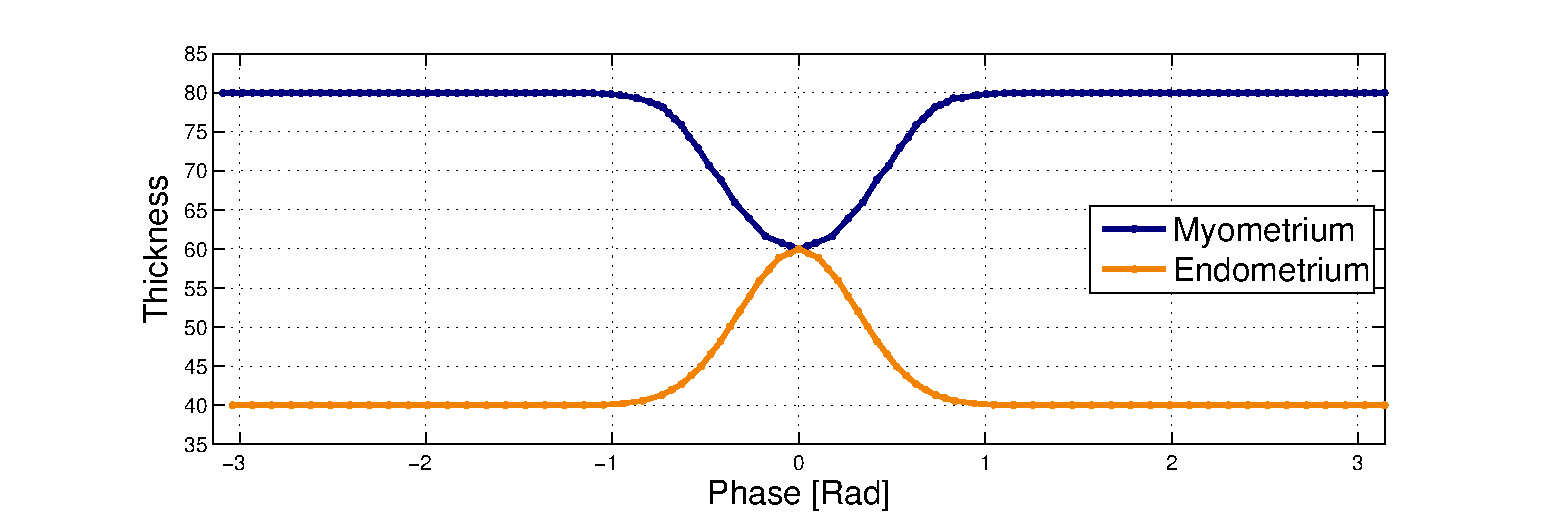
\includegraphics[width=8.3cm]{pics/synthWidth}}
  \centerline{(b)}\medskip
\end{minipage}
\caption{Results using synthetic curves. (a) Path traveled by points during the evolution. The blue lines corresponds to the evolution of the original points, while orange lines corresponds to created points. (b) Thickness profile relative to the angle measured from the center of the circles. In blue is shown the thickness of region between $\Gamma_1$ and $\Gamma_2$, and in orange between $\Gamma_2$ and $\Gamma_3$.}
\label{fig:synth}
\end{figure}

\subsection{Real}
\label{ssec:real}
Postpartum uterine diseases, such as endometrium damage and ovarian cyclic activity disruption, has become one of the most important causes of reproductive inefficiency in dairy cattle and are associated with infertility \cite{sheldon2008,barlund2008}. Endometritis is an uterine disease defined as inflammation limited to the endometrium occurring at least 21 days after calving and not associated with systemic illness \cite{sheldon2010}. This disease do not always presents clinical symptoms, so sub-clinical Endometritis detection using ultrasonography images is used \cite{Gianni2010, Gianni2013}. The sub-clinical endometritis diagnostic is very difficult, even for an expert, so image processing techniques to aid veterinaries in diagnostics get special relevance.

In this section we present results obtained in real ultrasonography images. The curves were manually segmented by the expert and our algorithm applied to obtain the thickness profile. Results are shown in Figure \ref{fig:real} for three real examples.

\subsection{Feature extraction and classification}
\label{ssec:clasification}
The algorithm was applied to a database tagged by the expert, knowing which cows has sub-clinical endometritis. In a preliminary study of the problem the thickness obtained for each image was used to obtain some descriptors in order to perform an automatic supervised classification of cattle with or without endometritis. Although the results are preliminary, seems to be very promissory. With the descriptors used, we were able to detect 88\% of infected cows. \textcolor{red}{habria que explicar mejor todo esto?}. This results are showing that descriptors obtained from the thickness profile, which could not be extracted using other measures such as euclidean distance, can play an important role in detecting sub-clinical endometritis.

\begin{figure*}[t]
\begin{minipage}[b]{.33\linewidth}
  \centering
  \centerline{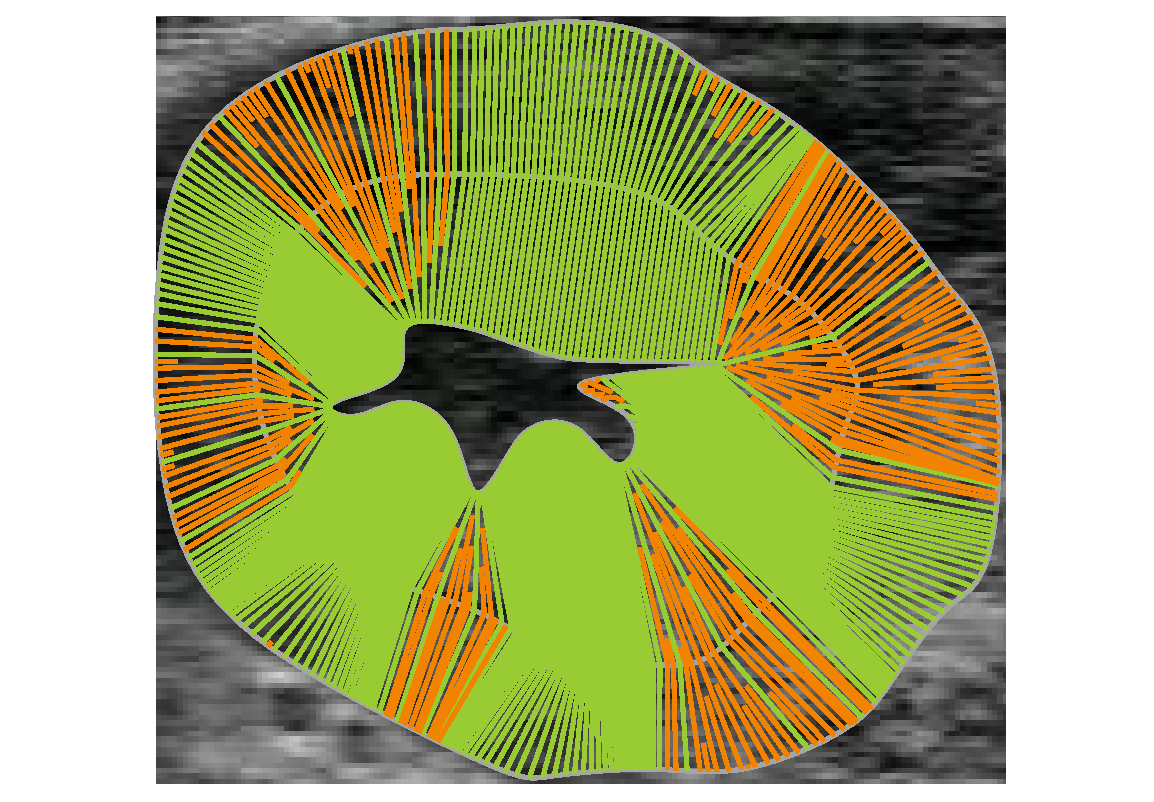
\includegraphics[width=6.5cm]{pics/real}}
  \centerline{(a) Evolution}\medskip
\end{minipage}
\hfill
\begin{minipage}[b]{.33\linewidth}
  \centering
  \centerline{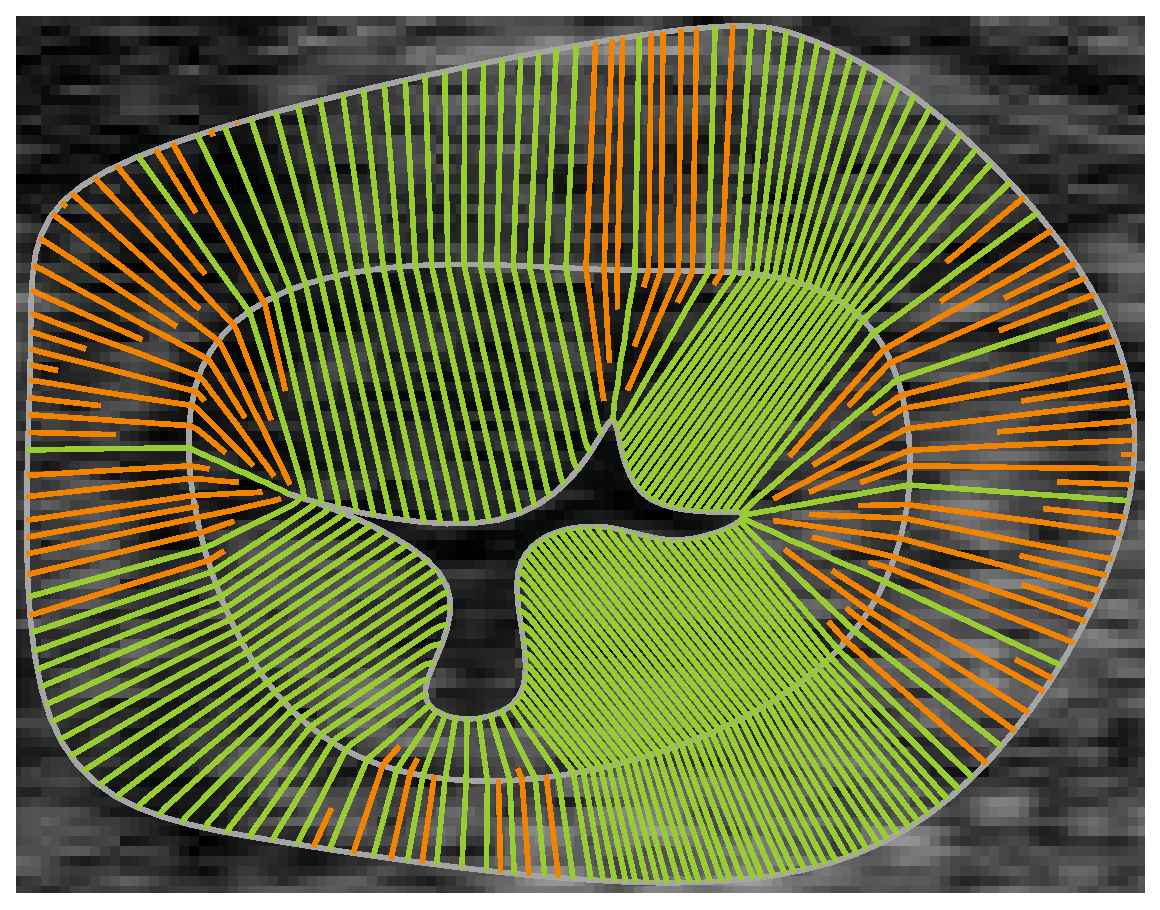
\includegraphics[width=6.5cm]{pics/real4}}
  \centerline{(c) Evolution}\medskip
\end{minipage}
\hfill
\begin{minipage}[b]{.33\linewidth}
  \centering
  \centerline{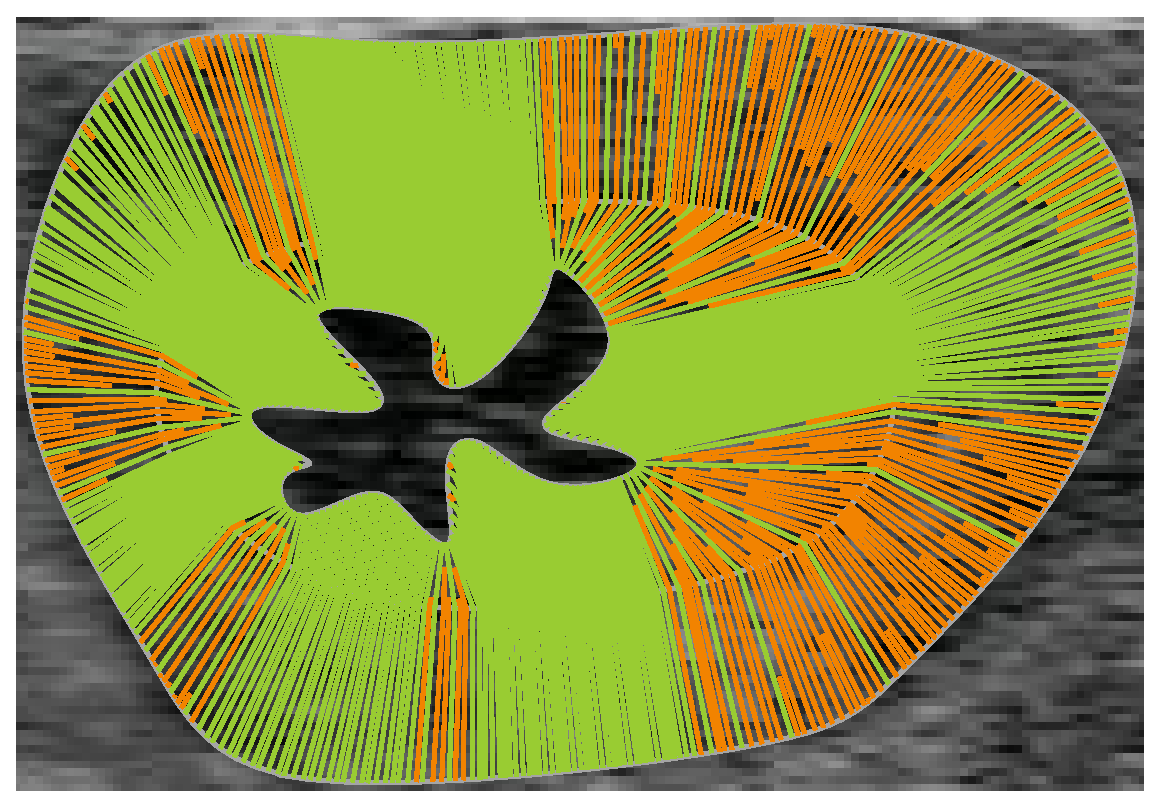
\includegraphics[width=6.5cm]{pics/real3}}
  \centerline{(e) Evolution}\medskip
\end{minipage}
\hfill
\begin{minipage}[b]{.33\linewidth}
  \centering
  \centerline{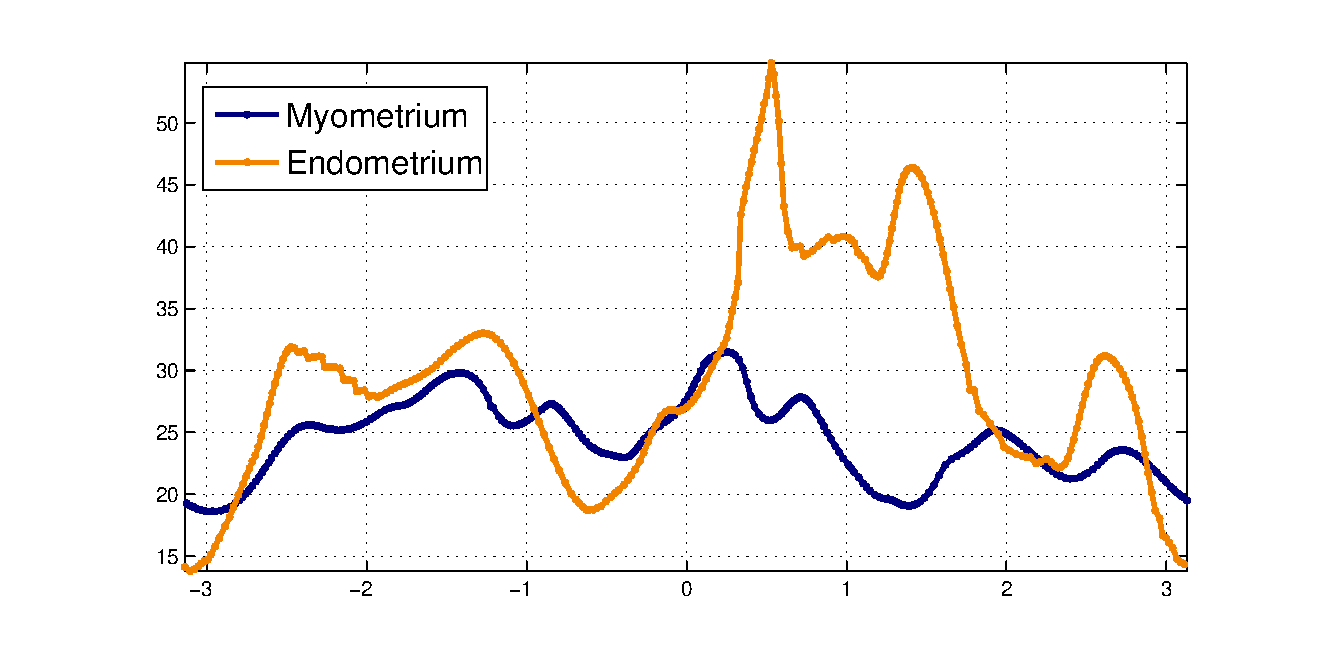
\includegraphics[width=6.5cm]{pics/realWidth}}
  \centerline{(b) Evolution}\medskip
\end{minipage}
\hfill
\begin{minipage}[b]{.33\linewidth}
  \centering
  \centerline{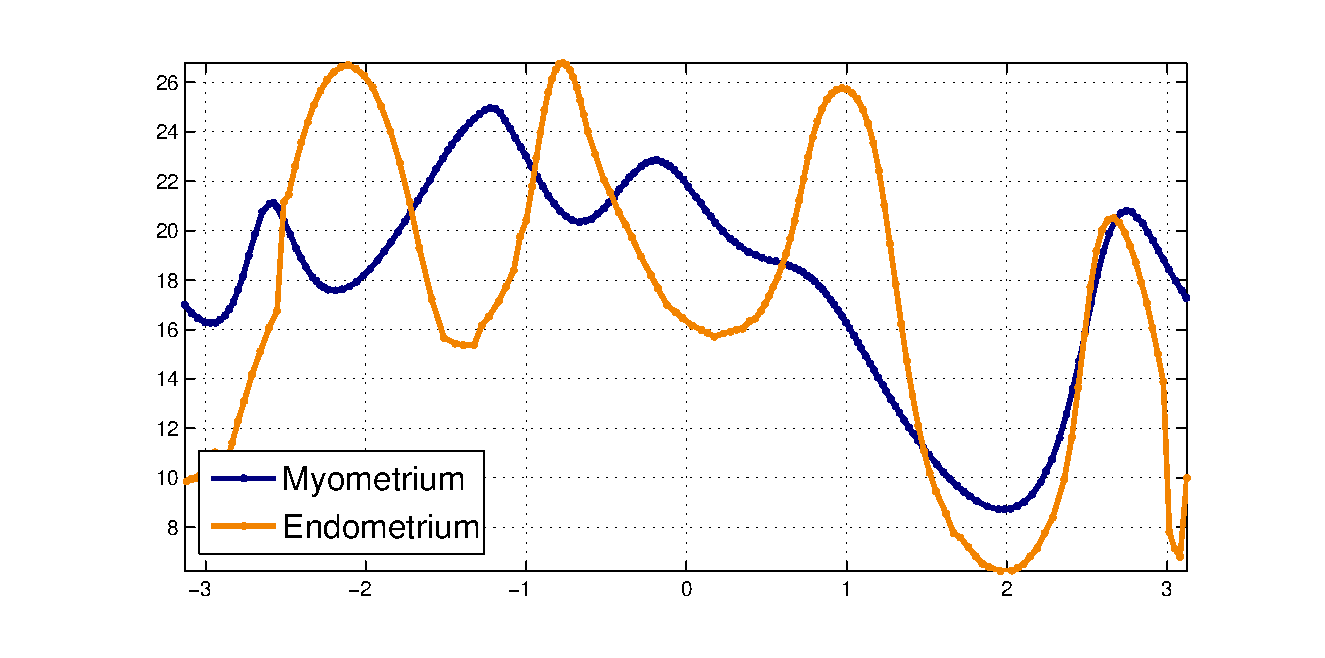
\includegraphics[width=6.5cm]{pics/realWidth4}}
  \centerline{(d) Evolution}\medskip
\end{minipage}
\hfill
\begin{minipage}[b]{.33\linewidth}
  \centering
  \centerline{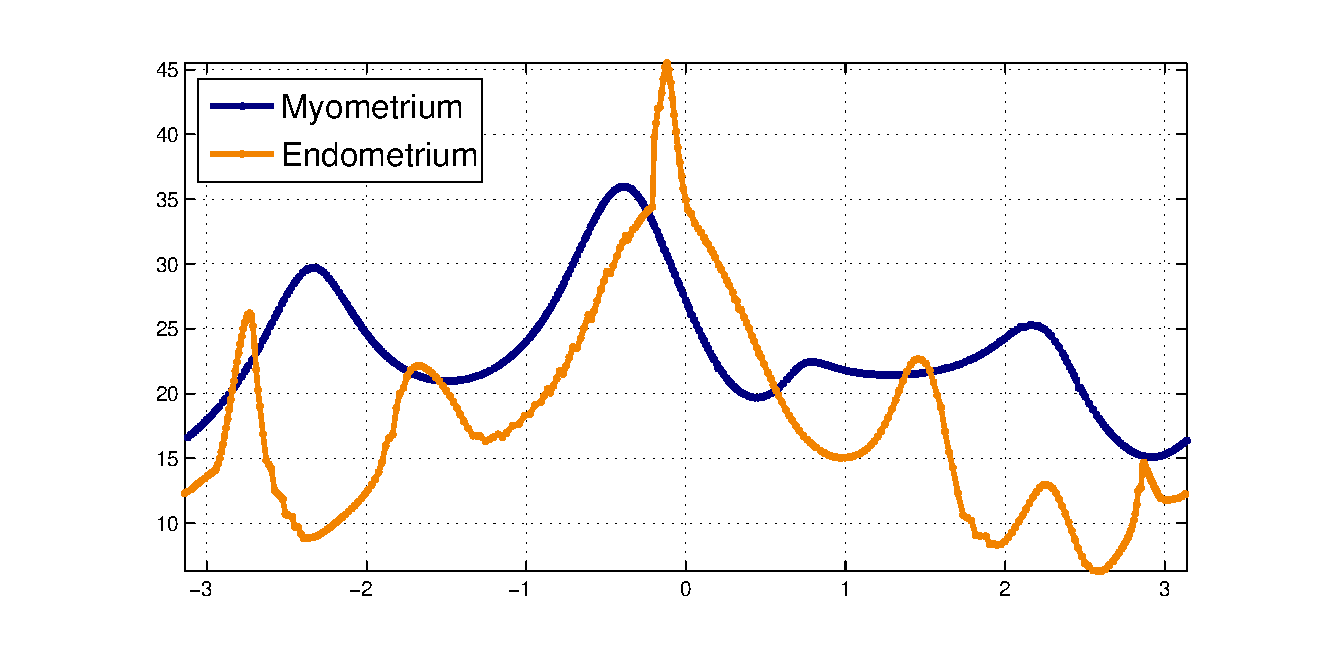
\includegraphics[width=6.5cm]{pics/realWidth3}}
  \centerline{(f) Evolution}\medskip
\end{minipage}
\caption{Real results.}
\label{fig:real}
\end{figure*}


\section{Conclusion}
\label{sec:conc}
In this work we present an algorithm to measure the thickness of a region delimited by two closed curves, without any regularity assumptions on the curves. The curves are sampled according to curvature and the algorithm is based on the normal evolution with constant velocity of the points of the curve to evolve. Mechanisms of creating and deleting points during evolution were designed and implemented, ensuring a good representation of the curve in each step. To deal with the ``irregularity'', meaning the high variation of curvature of a curve, the convex hull is considered as an auxiliary curve and the evolution is performed in two steps: evolving from the convex hull to the origin curve and evolving from the convex hull to the target curve. This algorithm leads to an intuitive thickness definition, and an entire thickness profile is obtained. When defining the thickness, the correspondence between the curves is not clear, but this algorithm finds a reasonable correspondence, resolving an entire mapping between curves. Also, it is important to mention that the algorithm is fast and efficient.

The algorithm was applied to a particular problem, where the goal is to measure the thickness of a muscle of cattle uterus. This thickness appears to be very relevant to help the detection of a sub-clinical uterine disease: endometritis. Some descriptors were extracted from the thickness profile, and a simple classification system was implemented in order to classify sick cows. The results are very promissory, giving good prospects for automatic detection.

\subsection{Future work}
\label{ssec:future}
As future work we plan to explore in extracting better descriptors from the thickness profile and obtain other descriptors from the ultrasonographic images, such as texture or shape descriptors, in order to obtain a more accurate classification. Also we plan to enlarge the database.

\bibliographystyle{IEEEbib}
\bibliography{refs}

\balance

\end{document}

% To start a new column (but not a new page) and help balance the last-page
% column length use \vfill\pagebreak.
% -------------------------------------------------------------------------
%\vfill
%\pagebreak

% Below is an example of how to insert images. Delete the ``\vspace'' line,
% uncomment the preceding line ``\centerline...'' and replace ``imageX.ps''
% with a suitable PostScript file name.
% -------------------------------------------------------------------------
\begin{figure}[t]

\begin{minipage}[b]{1.0\linewidth}
  \centering
  \centerline{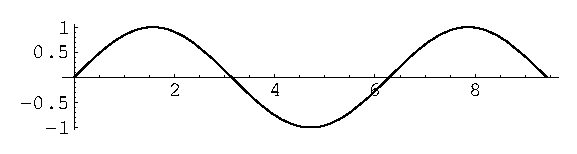
\includegraphics[width=8.5cm]{pics/image1}}
%  \vspace{2.0cm}
  \centerline{(a) Result 1}\medskip
\end{minipage}
%
\begin{minipage}[b]{.48\linewidth}
  \centering
  \centerline{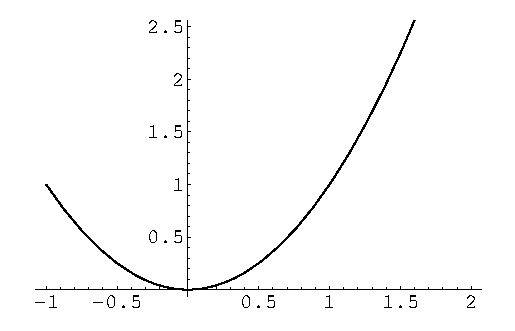
\includegraphics[width=4.0cm]{pics/image3}}
%  \vspace{1.5cm}
  \centerline{(b) Results 3}\medskip
\end{minipage}
\hfill
\begin{minipage}[b]{0.48\linewidth}
  \centering
  \centerline{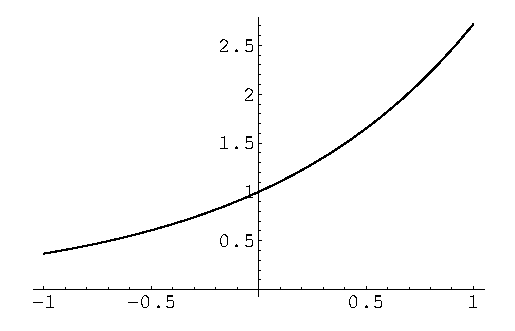
\includegraphics[width=4.0cm]{pics/image4}}
%  \vspace{1.5cm}
  \centerline{(c) Result 4}\medskip
\end{minipage}
%
\caption{Example of placing a figure with experimental results.}
\label{fig:res}
%
\end{figure}
